% tricl methods paper.  Build: see README.md in this directory.
\documentclass[11pt,a4paper]{article}

\usepackage[utf8]{inputenc}
\usepackage[T1]{fontenc}
\usepackage{lmodern}
\usepackage[margin=2.5cm]{geometry}
\usepackage{amsmath,amssymb}
\usepackage{graphicx}
\usepackage{booktabs}
\usepackage{xcolor}
\usepackage{listings}
\usepackage{tikz}
\usetikzlibrary{arrows.meta,positioning,calc}
\usepackage[numbers,sort&compress]{natbib}
\usepackage[hidelinks]{hyperref}
\usepackage{microtype}

% Notation and listing style.
\newcommand{\tricl}{\textsf{tricl}}
\newcommand{\R}{\mathbb{R}}
\newcommand{\E}{\mathbb{E}}
\newcommand{\expit}{\operatorname{expit}}
\newcommand{\ttt}[1]{\texttt{#1}}
\newtheorem{proposition}{Proposition}
\newtheorem{lemma}{Lemma}

\definecolor{codegray}{HTML}{52514E}
\lstdefinelanguage{yaml}{
  keywords={},
  comment=[l]{\#},
  morestring=[b]",
}
\lstset{
  basicstyle=\ttfamily\footnotesize,
  commentstyle=\color{codegray}\itshape,
  columns=fullflexible,
  keepspaces=true,
  frame=lines,
  framesep=4pt,
  xleftmargin=0pt,
  aboveskip=8pt,
  belowskip=8pt,
  literate={~}{{\textasciitilde}}1,
}

% generated by paper/make_figures.py -- do not edit
\newcommand{\AtopAone}{0.0102}
\newcommand{\AtopAzero}{\ensuremath{1.78\times 10^{-4}}}
\newcommand{\AtopCensored}{1\,707}
\newcommand{\AtopDropAone}{9\,314}
\newcommand{\AtopDropBone}{776}
\newcommand{\AtopEvalSeconds}{0.06}
\newcommand{\AtopEvents}{4\,514}
\newcommand{\AtopFormationRatio}{58}
\newcommand{\AtopHazFive}{0.035}
\newcommand{\AtopHazTwentySix}{0.0022}
\newcommand{\AtopHazZero}{0.054}
\newcommand{\AtopIntervals}{3\,000}
\newcommand{\AtopLifeZero}{18}
\newcommand{\AtopProfileGap}{891}
\newcommand{\AtopShuffleAone}{4}
\newcommand{\AtopShuffleAzero}{28}
\newcommand{\AtopShuffleBone}{1}
\newcommand{\AtopStates}{217}
\newcommand{\MacroGranOde}{30}
\newcommand{\MacroGranSim}{38}
\newcommand{\MacroSiOde}{271}
\newcommand{\MacroSiSim}{165}
\newcommand{\RecoveryCovMax}{1.00}
\newcommand{\RecoveryCovMin}{0.90}
\newcommand{\RecoveryEvents}{1040}
\newcommand{\RecoverySeeds}{40}
\newcommand{\RecoveryT}{400}
\newcommand{\TestSigmoidChecks}{81\,063}


\title{tricl: likelihood-based simulation and inference for\\ typed multi-relational network dynamics}
\author{Jobst Heitzig\\[2pt] \small Potsdam Institute for Climate Impact Research, Potsdam, Germany}
\date{Draft, \today}

\begin{document}
\maketitle

\begin{abstract}
Many social, economic and political systems are networks of several kinds of entities linked by
several kinds of relationships that form and dissolve over time, at rates that depend on the
surrounding network: friends of friends become friends, states ally with their allies' allies,
agents adopt a behaviour when enough contacts have adopted it. We present \tricl, an open-source
simulator and inference engine for such dynamics. A model is a short configuration file that
declares entity types, relationship types and rules saying how the attempt rate and the success
probability of establishing or terminating a link depend on the numbers of adjacent two-paths of
each type. States of entities and well-mixed interactions are expressed with the same rule language
by links to auxiliary entities. The resulting continuous-time Markov chain is simulated exactly with
Gillespie's direct method over a sum tree of event rates. Because every rule enters the rates
explicitly, \tricl\ also computes the exact log-likelihood of an observed event sequence and its
gradient with respect to all model parameters, which turns the simulator into a maximum-likelihood
estimator; it further generates mean-field equations from the same file. We describe the model
class, the algorithms and their tests, and show parameter recovery, the mean-field approximation
and a first application: the formation and dissolution of defense pacts between states from 1816 to
2018, where a common ally raises the rate of pact formation about \AtopFormationRatio-fold.
\end{abstract}

\section{Introduction}\label{sec:intro}

Wearable proximity sensors record face-to-face contacts between people at a resolution of seconds \citep{cattuto2010,stehle2011}, and the resulting temporal networks \citep{holme2012} have become a standard empirical basis for models of social contact and epidemic spreading.
Their most robust statistical feature is the broad distribution of contact durations and of the intervals between successive contacts of the same pair, far from the exponential distributions of a memoryless process.
The prevailing explanation is an intrinsic memory of the individuals: the probability to leave a contact or a group decreases with the time already spent in it, as in the reinforcement models of \citet{zhao2011} and \citet{starnini2013}, or ties are reinforced by repeated interaction, as in activity-driven networks with memory \citep{karsai2014}.
Such aging makes the process non-Markovian in the network state.

An alternative explanation is that the process is Markovian, but in a richer state than the set of current contacts.
A contact embedded in a group (with common contacts), between members of the same class, between friends, or of a student who currently has many other contacts, may have very different rates of ending than an isolated contact between strangers, and a mixture of such rates, changing as groups form and dissolve, also produces broad durations.
Traces of recent interactions that decay over time add memory to such a description while keeping it Markovian in an extended state, since the traces are part of the state.
The two explanations have different consequences: intrinsic aging puts the memory into the individuals, network context puts it into the configuration around them, and only the latter is captured by models of network structure.

Here we quantify how much of the memory is network context.
We specify a hierarchy of Markovian models with increasing context and memory, and a competing non-Markovian aging model, for the contacts of \Students\ students of a high school \citep{mastrandrea2015}, fit all models by maximum likelihood on three days, and compare them on two held-out days by their log-likelihood and by time-rescaling residuals \citep{brown2002}.
The Markovian models are rule sets for \tricl, a simulator and inference engine for typed multi-relational network dynamics, which computes the exact log-likelihood and its gradient for each rule set, including rates that decay between events.

We find that memory dominates and that network context explains only a small part of it, but that a Markovian model with decaying traces on several time scales outperforms power-law aging.
We also find that all fitted models with network feedback are dynamically unstable, a form of model degeneracy that a pair closure of the generated mean-field equations predicts and a standard closure misses.
Section~\ref{sec:data} describes the data, Sec.~\ref{sec:models} the models, Sec.~\ref{sec:inference} inference and evaluation, Sec.~\ref{sec:results} the results, Sec.~\ref{sec:closure} the stability analysis and closures, and Sec.~\ref{sec:discussion} the conclusions.

\section{Model class}\label{sec:model}

\subsection{State}
A \tricl\ model has a finite set of \emph{entities}, each of one \emph{entity type}, and a finite set of \emph{relationship types}.
The state at time $t$ is a set $G(t)$ of \emph{links} $\ell = (e_1, r, e_3)$, each a directed edge of relationship type $r$ from entity $e_1$ to entity $e_3 \neq e_1$.
A relationship type may be declared \emph{symmetric} (e.g.\ \ttt{knows}) or have a named \emph{inverse} (\ttt{follows}/\ttt{is followed by}); then every link implies its mirrored link, and the two are established and terminated together.
A built-in identity relationship ``='' links every entity to itself and never changes; it lets rules refer to an existing link between the two entities, or to a link of one of them to a third entity of a given kind, with the same syntax as to two-paths.
Apart from the identity relationship there are no self-links, as in the original implementation: a self-link $(e_1, r, e_1)$ would turn every link $(e_1, r', e_3)$ into a two-path $e_1 \xrightarrow{r} e_1 \xrightarrow{r'} e_3$ of the same type as a two-path through a third entity, so that, e.g., an existing acquaintance would count as a common acquaintance; states of entities are encoded by links to auxiliary entities instead (Sec.~\ref{sec:expressiveness}).
The \emph{link type} of $\ell$ is the triple (type of $e_1$, $r$, type of $e_3$).

\subsection{Events and rates}
An \emph{event} establishes a link that does not exist or terminates one that exists.
For a candidate link $\ell = (e_1, r, e_3)$, an \emph{angle} is a two-path $e_1 \xrightarrow{r_{12}} e_2 \xrightarrow{r_{23}} e_3$ in $G(t)$ with $r_{12}, r_{23}$ including the identity relationship; its \emph{angle type} is $(r_{12}, \text{type of } e_2, r_{23})$.
For every event type $\tau$ (establish or terminate, link type), the configuration file specifies a basic attempt rate $a^0_\tau \ge 0$, basic success \emph{probability units} $b^0_\tau \in \R \cup \{\pm\infty\}$, and for any angle type $k$ an additional attempt rate $a_{\tau k}$ and additional probability units $b_{\tau k}$ contributed by each adjacent angle of that type.
With $n_k(\ell, t)$ the number of angles of type $k$ adjacent to $\ell$ at time $t$, the event happens at rate
\begin{equation}\label{eq:rate}
\begin{aligned}
  \lambda_\tau(\ell, t) &= A \cdot f(B), \\
  A &= a^0_\tau + \textstyle\sum_k a_{\tau k}\, n_k(\ell,t), \\
  B &= b^0_\tau + \textstyle\sum_k b_{\tau k}\, n_k(\ell,t),
\end{aligned}
\end{equation}
i.e.\ attempts occur at the rate $A$ and succeed with probability $f(B)$.
Coefficients may be expressions of named \emph{metaparameters}, which can be overridden on the command line and are the parameters estimated in Sec.~\ref{sec:inference}.
Infinite coefficients encode logic: a contribution $-\infty$ to $B$ makes the event impossible, and an infinite attempt rate with positive success probability makes it \emph{immediate}; all pending immediate events are performed, in a uniformly random order, before time advances.
Immediate events implement state machines: if an agent acquires a link \ttt{is infectious for} to the entity \ttt{covid-19}, the rule ``terminate \ttt{is susceptible to} immediately when the angle \ttt{is infectious for}, \ttt{covid-19}, = exists'' removes its previous state.

\subsection{The sigmoid}
The success probability is a sigmoid $f$ of the probability units with two \emph{tail indices} $\sigma_0, \sigma_1 \ge 0$ that set how fast it approaches $0$ and $1$:
\begin{equation}\label{eq:sigmoid}
\begin{aligned}
  f(B) &= \tfrac12 T_{\sigma_0}(-v) + \tfrac12 - \tfrac12 T_{\sigma_1}(v), \quad
  v = \frac{4B}{k(\sigma_0) + k(\sigma_1)}, \\
  T_\sigma(x) &= \bigl(1 + \sigma \ln(1 + e^{x})\bigr)^{-1/\sigma}, \quad T_0(x) = \frac{1}{1+e^{x}}, \\
  k(\sigma) &= (1 + \sigma\ln 2)^{-1-1/\sigma}, \quad k(0) = \tfrac12.
\end{aligned}
\end{equation}
$T_\sigma$ replaces the exponential tail of the logistic function by the $q$-exponential $(1 + \sigma y)^{-1/\sigma}$ of $y = \ln(1+e^{x})$ \citep{tsallis1988}.
For $\sigma > 0$ the tail decays like $|B|^{-1/\sigma}$, for $\sigma = 0$ exponentially.
Since $k(\sigma) = -2T'_\sigma(0)$, $f$ has slope $1$ at $B = 0$ for all tail indices, so that near zero, probability units are differences of probabilities. $f$ is strictly increasing, continuous in the tail indices, and equals $\expit(4B)$ for $\sigma_0 = \sigma_1 = 0$.
Heavy tails (the default is $\sigma_0 = \sigma_1 = 1$) keep rare events possible when many angles push the probability units far from zero.

\subsection{A model file}
The following excerpt is the dynamics of a model of triadic closure with triangle stabilization in three blocks of 100 entities (the \ttt{parameters\_3blocks} example):
\begin{lstlisting}[language=yaml]
relationship types:
  knows: symmetric
dynamics:
  [user, knows, user]:
    establish:
      attempt:
        basic: 0.001                     # spontaneous
        [~, knows, user, knows, ~]: 0.01 # per common
      success:                           # acquaintance
        basic: .inf                      # always succeed
    terminate:
      attempt:
        basic: 10.0                      # fast decay ...
      success:                           # ... hampered
        [~, knows, user, knows, ~]: -0.3 # by triangles
\end{lstlisting}
\noindent The angle type \ttt{[\~{}, knows, user, knows, \~{}]} counts common acquaintances. Further
sections of the file declare entity types and numbers, named entities, and initial links, which can be listed, read from csv files, or drawn from random graph models (Erd\H{o}s--R\'enyi, block models, random geometric graphs).

\subsection{Expressiveness}\label{sec:expressiveness}
Entity states are links to auxiliary ``hub'' entities: an agent is active if it has the link \ttt{is}~\ttt{active}.
A rule on the angle (agent, \ttt{knows}, agent, \ttt{is}, \ttt{active}) then depends on the number of active neighbors, which yields threshold models \citep{granovetter1978,wiedermann2020} (Fig.~\ref{fig:frames}) and contact processes; angles through ``='' make rates depend on an entity's own state, which yields compartmental epidemic models on adaptive networks \citep{gross2006}, including social distancing as termination of contacts with infectious agents.
Structural balance dynamics \citep{heider1946,antal2005} needs two relationship types \ttt{likes} and \ttt{dislikes} and four angle rules.
Well-mixed interactions are angles through a hub to which all entities are linked.
What is outside the class: rates that depend on structures beyond two-paths (e.g.\ on cycles of length four) and rates that depend on time or on the history of the process.
Rules on single links of one endpoint (``legs'', which would make rates depend on degrees) are part of the configuration syntax but rejected by the current version.

\section{Simulation}\label{sec:simulation}

\subsection{Algorithm}
The process is a continuous-time Markov chain with finitely many possible events, so it can be
simulated exactly by drawing the waiting time until the next event from an exponential distribution
with the total rate and then choosing the event with probability proportional to its rate
\citep{gillespie1977,bortz1975}. The number of possible events grows quadratically with the number of
entities, but in sparse networks most of them are spontaneous establishments of links between
entities without any adjacent angle, whose rates are equal within an event type. \tricl\ therefore
schedules three kinds of events:
\begin{itemize}
\item \emph{Individual events}: all terminations of existing links and all establishments with at
  least one adjacent angle of an influencing type. Their rates are the leaves of a complete binary
  \emph{sum tree}, whose inner nodes hold the sums of their children. Updating a rate costs
  $O(\log n)$ for $n$ scheduled events; the root holds the total, and choosing an event with
  probability proportional to its rate is a descent from the root.
\item \emph{Summary events}, one per type of spontaneous establishment, which stand for all pairs of
  entities of the two types. A summary event's leaf holds the upper bound
  $a^0_\tau p^{\max}_\tau N_1 N_3$, with $N_1, N_3$ the numbers of entities of the two types and
  $p^{\max}_\tau$ the largest success probability a covered pair can have. When it is chosen, a pair is
  drawn uniformly; the attempt is discarded if the pair is identical, already linked or scheduled
  individually, and otherwise succeeds with probability $f(B)/p^{\max}_\tau$. This is thinning in the
  sense of \citet{lewis1979}: proposals arrive at the upper-bound rate and are accepted with the ratio
  of the true to the bounding rate, which yields exactly the true rate for every pair.
\item \emph{Immediate events} (infinite rates) are kept in a separate list. While it is not empty,
  one of its events is drawn uniformly and performed without advancing time.
\end{itemize}
After an event on the pair $(e_1, e_3)$, only events whose angle counts change need new rates: those
of pairs $(e_1', e_3)$ with a link between $e_1'$ and $e_1$, and of pairs $(e_1, e_3')$ with a link
between $e_3$ and $e_3'$, for the relationship types that occur in rules. The cost per event is thus
$O\bigl((d_1 + d_3) \log n\bigr)$ in the degrees $d_1, d_3$ of the endpoints. Adjacent angles are found
by intersecting the sorted link sets of the two endpoints, with a galloping search when one set is
much larger than the other, so that the intersection costs time proportional to the smaller set
times the logarithm of the larger one; a hub entity linked to all others (the usual encoding of
states) therefore does not make every event cost time linear in the number of entities. An earlier version scheduled events by
tentative times in an ordered map \citep{gibson2000}; the direct method needs two random numbers per
event instead of one per rate change and gives the exact total rate at all times, which the
likelihood (Sec.~\ref{sec:inference}) needs.

\subsection{Tests}
The test suite runs in continuous integration in optimized, debug and sanitizer builds. It checks
the sigmoid (\TestSigmoidChecks\ unit checks of values, limits, monotonicity and derivatives), the
exact log-likelihood against a closed form for a two-entity model, analytic gradients against finite
differences, that replaying a simulated event sequence reproduces the simulation's log-likelihood,
and, in debug builds, the consistency of every scheduled rate with a recomputation from the
network. Replacing the scheduler left the distribution of all reported statistics unchanged within
sampling error (between 60 and 400 seeds per model; all $|z| < 1.6$).

\subsection{Performance}
Table~\ref{tab:benchmark} reports throughput on one core. Sparse models run at
$10^4$--$10^5$ events per second, and a hundredfold increase in the number of agents of the threshold
model reduces the throughput only about fourfold. In dense models every event changes the rates of
hundreds of others, so the throughput is limited by the number of rate updates. Memory use is a few
tens of megabytes for these models.

\begin{table}[t]
\caption{Throughput of \tricl\ on one core of a cloud virtual machine (best of three runs of
$2\times 10^4$ events, initialization excluded). Helfmann: threshold model of
Fig.~\ref{fig:frames} with mean degree 10; 3-blocks: the triadic-closure model of
Sec.~\ref{sec:model}, mean degree about 100; SIR: epidemic with social distancing on a random
geometric graph.}
\label{tab:benchmark}
\begin{tabular}{llrrr}
\toprule
model & agents & events & initialisation [s] & events per second \\
\midrule
Helfmann & 100 & 20\,000 & 0.07 & 245\,400 \\
Helfmann & 1\,000 & 20\,000 & 0.14 & 164\,600 \\
Helfmann & 10\,000 & 20\,000 & 2.25 & 62\,200 \\
3-blocks (dense) & 300 & 20\,000 & 1.08 & 2\,400 \\
SIR with distancing & 1\,000 & 7\,155 & 0.25 & 33\,000 \\
\bottomrule
\end{tabular}

\end{table}

\section{Inference and evaluation}\label{sec:inference}

\subsection{Exact log-likelihood}
For a fully observed sequence of events in a window $[0, T]$, the log-likelihood is
\begin{equation}\label{eq:logl}
  L(\theta) = \sum_i \ln \lambda_{\tau_i}(\ell_i, t_i^-; \theta) - \int_0^T \Lambda(t; \theta)\,dt,
\end{equation}
where $\Lambda$ is the total rate of all possible events.
\tricl\ maintains $\Lambda$ incrementally during a replay of the observed events, including the pairs without any adjacent angle, whose rates depend only on the degrees of their endpoints and which are summed through histograms of degree vectors.
Rates with decaying impacts vary continuously between events; their integrals are accumulated per event by Gauss--Legendre quadrature whenever the event's rate is updated (App.~\ref{app:likelihood}).
Forced events and acts triggered by contact events add no terms, so that $L$ is conditional on the timetable.
\tricl\ also computes the gradient of $L$ with respect to all coefficients, and we maximize $L$ with L-BFGS-B \citep{byrd1995}, summing over the training days, which are independent observation windows (the network is empty at the start of each day).

\subsection{Held-out likelihood and time rescaling}
We compare models by their log-likelihood on the held-out days, evaluated at the estimates from the training days, which penalizes overfitting directly.
As a goodness-of-fit test, we use the time-rescaling theorem \citep{brown2002}: if the model is correct, the integrated termination hazard $\Lambda$ of each contact from its start to its end is a unit exponential variable, independently across contacts.
\tricl\ outputs these integrals for the observed contacts, summed over both directions of a pair and including time-varying rates; we report the Kolmogorov--Smirnov distance of their distribution from the unit exponential distribution.
On simulated data from a known model with impacts and a timetable, the integrals are indeed unit exponential variables (a test of the implementation).

\subsection{Simulation}
\tricl\ simulates the models exactly with the direct method over a sum tree of rates; events with decaying rates are simulated by thinning \citep{lewis1979,ogata1981}, with upper bounds that are valid until the next update of each event, and forced events and the expiry of actions are processed at their times (App.~\ref{app:thinning}).

\section{Mean-field approximation}\label{sec:macro}

Because a model is a finite set of typed rules, its mean-field equations can be generated mechanically.
\ttt{tricl\_macro.py} reads the model structure from \ttt{tricl --dump-model} and takes as state variables the numbers $n_L$ of links of every link type $L$.
For a candidate link of type $L$ between entities of types $\alpha$ and $\gamma$, the number of adjacent angles of type $(r_{12}, \beta, r_{23})$ is approximated by a Poisson variable with mean $N_\beta\, \rho(\alpha, r_{12}, \beta)\, \rho(\beta, r_{23}, \gamma)$, independently across angle types, where $\rho$ is the current density of the respective link type.
Averaging the rates of Eq.~\eqref{eq:rate} over these distributions gives
\begin{equation}\label{eq:mf}
  \frac{dn_L}{dt} = (\text{unlinked pairs of type } L)\cdot\langle \lambda^{\text{est}}_L \rangle
                   - n_L \cdot \langle \lambda^{\text{term}}_L \rangle,
\end{equation}
with the necessary corrections for symmetric and inverse relationship types and for immediate events.
This is the pair-level mean-field closure of the adaptive-network literature \citep{gross2006,demirel2014}; for models whose rates do not depend on angles it is the exact equation for the expected counts (Appendix~\ref{app:meanfield}), and the law of large numbers for density-dependent Markov chains \citep{kurtz1970} then makes it the limit for large systems.

Figure~\ref{fig:macro} compares the approximation with simulations.
For linear state switching (no angle influences) it agrees within sampling error.
For an infection process on a random geometric graph it overestimates the prevalence substantially, because infections cluster in space and infected agents' neighbors are more often already infected than the closure assumes; for the threshold model it underestimates the number of active agents.
The generated equations thus provide a baseline whose deviation from the simulation measures the effect of link correlations, and a starting point for higher-order closures \citep{gleeson2011,demirel2014}.

\begin{figure*}[t]
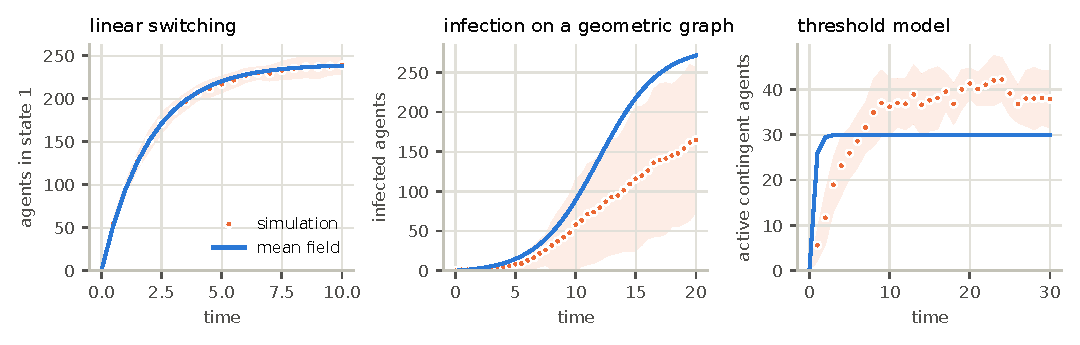
\includegraphics[width=\textwidth]{generated/fig-macro}
\caption{Automatically generated mean-field approximation (lines) and simulations (mean and $\pm 1$ standard deviation over seeds, markers and bands).
Left: 400 agents switching independently between two states (20 seeds).
Middle: infection with recovery on a random geometric graph of 1000 agents (10 seeds).
Right: number of active contingent agents in the threshold model of Fig.~\ref{fig:frames} (10 seeds).}
\label{fig:macro}
\end{figure*}

\section{Application: military alliances 1816--2018}\label{sec:application}

\subsection{Data and model}
The Alliance Treaty Obligations and Provisions project \citep{leeds2002} records for every pair of states and year whether an alliance with a defense pledge was in effect; we use version 5.1 as distributed with the R package \texttt{peacesciencer} \citep{miller2022}, together with the Correlates of War list of state system members (version 2016).
Every maximal run of consecutive years in which a pair has a defense pledge becomes one interval of a symmetric link \ttt{defense}, established at the start of its first year and terminated at the start of the year after its last one.
Membership of a state in the international system is a link \ttt{[state, is in, system]} to a single hub entity.
This gives \AtopStates\ states, \AtopIntervals\ pact intervals (\AtopCensored\ still in effect in 2018) and \AtopEvents\ events (Fig.~\ref{fig:atop}, left).
The model has six metaparameters:
\par\noindent\begin{minipage}{\linewidth}
\begin{lstlisting}[language=yaml]
[state, defense, state]:
  establish:
    attempt:
      [~, is in, system, contains, ~]: a0  # per direction
      [~, defense, state, defense, ~]: a1  # per ally
    success: inf
  terminate:
    attempt:
      base: d0
    success:
      tails: 0
      [~, defense, state, defense, ~]: -b1 # per ally
[state, is in, system]: rates "entry", "exit"
\end{lstlisting}
\end{minipage}
\noindent Formation thus needs both states to be members (the angle through the hub), and its rate
grows linearly in the number of common allies; dissolution attempts succeed with probability $\expit(-4 b_1 k)$ for $k$ common allies.
Since \ttt{defense} is symmetric, both directed links of a pair are possible events with these rates, so a pair of member states forms a pact at the rate $2(a_0 + a_1 k)$ and a pact dissolves at the hazard $2 d_0 \expit(-4 b_1 k)$ (Sec.~\ref{sec:model}).

Two features of the data need a convention.
Pledges are recorded per year, so events of the same year are simultaneous; we order them as terminations, exits, entries, formations, and formations by state codes.
And a multilateral treaty appears as many dyadic events in one year, so that the later ones already see the earlier ones as common allies.
With a random order of the events within a year, the estimates change by the amounts discussed below.

\subsection{Results}
Table~\ref{tab:atop} reports the maximum-likelihood estimates.
A pair of member states without a common ally forms a pact at a rate of $2a_0 = \AtopPairAzero$ per year; each common ally adds $2a_1 = \AtopPairAone$, so that one common ally raises the formation rate about \AtopFormationRatio-fold.
The dissolution hazard is $2 d_0\,\expit(-4 b_1 k)$: \AtopHazZero\ per year without common allies (a mean pact duration of \AtopLifeZero\ years), \AtopHazFive\ with five and \AtopHazTwentySix\ with 26, the size of NATO in 2004 (Fig.~\ref{fig:atop}, right).
Both effects are strongly supported: removing the ally-of-ally term from the formation rule lowers the maximal log-likelihood by \AtopDropAone, removing the stabilization term by \AtopDropBone.
With a random order of the simultaneous events, $a_0$ changes by \AtopShuffleAzero\%, $a_1$ by \AtopShuffleAone\% and $b_1$ by \AtopShuffleBone\%, so the formation effect partly reflects treaty-level events, which a model with an explicit treaty entity type could separate.

The profile log-likelihood of $b_1$ (Fig.~\ref{fig:atop}, middle) is not unimodal. Below a local minimum at small negative values it rises again towards a plateau as $b_1 \to -\infty$, where any common ally makes every dissolution attempt succeed; the plateau lies about \AtopProfileGap\ log-likelihood units below the maximum.
An optimizer started at negative values drifts towards the plateau, which illustrates the non-concavity in the probability units noted in Sec.~\ref{sec:inference}; the generated model therefore starts the fit at a positive value.
A likelihood evaluation of the \AtopEvents\ events takes about \AtopEvalSeconds\ seconds, a complete fit with standard errors about a minute.

\begin{table*}[t]
\caption{Maximum-likelihood estimates for the alliance model (standard errors from the observed information).
Rates per year.}
\label{tab:atop}
\begin{tabular}{llrr}
\toprule
parameter & meaning & estimate & s.e. \\
\midrule
$a_0$ & formation rate per pair of member states & $1.78\times 10^{-4}$ & $8.2\times 10^{-6}$ \\
$a_1$ & additional formation rate per common ally & $0.0102$ & $2.0\times 10^{-4}$ \\
$d_0$ & dissolution attempt rate & $0.108$ & $0.0048$ \\
$b_1$ & probability units per common ally (dissolution) & $0.0371$ & $9.2\times 10^{-4}$ \\
entry & entry rate of states & $0.00806$ & $5.4\times 10^{-4}$ \\
exit & exit rate of states & $0.00315$ & $4.4\times 10^{-4}$ \\
\midrule
\multicolumn{2}{l}{log-likelihood} & \multicolumn{2}{r}{$-20\,841.2$} \\
\bottomrule
\end{tabular}

\end{table*}

\begin{figure*}[t]
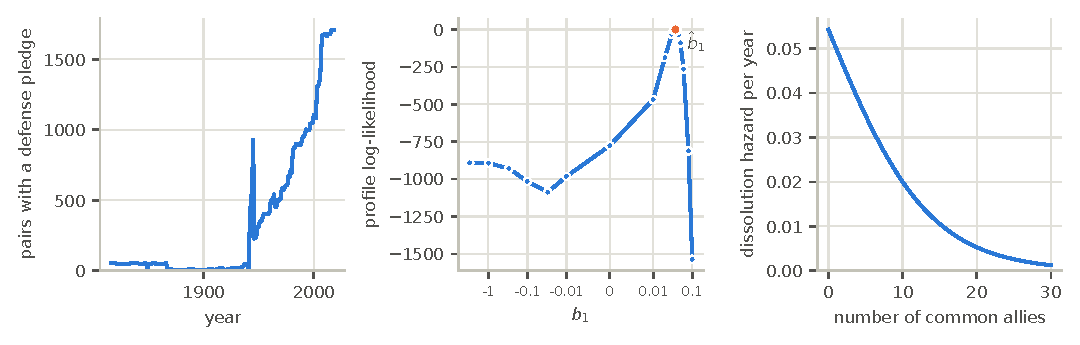
\includegraphics[width=\textwidth]{generated/fig-atop}
\caption{Defense pacts between states.
Left: number of pairs of states with a defense pledge in effect, per year.
Middle: profile log-likelihood of the stabilization parameter $b_1$ (all other parameters re-estimated), relative to its maximum (symmetric-log horizontal axis).
Right: estimated dissolution hazard as a function of the number of common allies.}
\label{fig:atop}
\end{figure*}

\section{Discussion}\label{sec:discussion}

\paragraph{Relation to other model families.}
Stochastic actor-oriented models \citep{snijders2001,snijders2010,snijders2017} describe network
change by actors who reconsider one outgoing tie at a time according to an objective function, and
are estimated from panel data by the method of moments or by likelihood-based methods with data
augmentation \citep{koskinen2007}. Relational event models \citep{butts2008} and dynamic network actor
models \citep{stadtfeld2017} model sequences of time-stamped interactions with rates that depend on
statistics of the past. \tricl\ is tie-oriented rather than actor-oriented: each potential link has
its own establishment and termination rates, which depend on the current two-path structure. It
shares with relational event models the exact likelihood of a fully observed event sequence, and
with the adaptive-network literature \citep{gross2008} the coupling of states and ties, which it
expresses within the same rule language through hub entities. Its distinctive features are typed
multi-relational networks with symmetric and inverse relationship types, models as configuration
files, immediate events for state logic, and the derivation of simulation, likelihood and mean-field
equations from the same file. The interval output of a run is a temporal network
\citep{holme2012} in the edge-list form that temporal-network software reads, and a mapping to the
Resource Description Framework (entity types as classes, relationship types as properties,
symmetric and inverse types as their OWL counterparts, link intervals as annotated triples) lets
\tricl\ import typed graphs from knowledge bases and export trajectories to them.

\paragraph{Limitations.}
Estimation requires a complete event sequence, including the timing of events. Most network data are
snapshots or panels; for them the likelihood is an integral over unobserved paths, which needs
simulation-based methods such as data augmentation or the method of simulated moments, both of which
the fast simulator makes feasible but which are not implemented yet. The rule language covers
two-path dependence only, and the coefficients do not depend on time; rules on single links of one
endpoint (degree dependence) are part of the syntax but not yet supported. The mean-field closure
ignores correlations between links (Section~\ref{sec:macro}). In the application, the yearly
resolution and the dyadic coding of multilateral treaties make the formation effect partly a
property of treaties rather than of pairs.

\paragraph{Outlook.}
Next steps are higher-order (pair and triple) closures generated in the same way, estimation from
snapshot data, rules on single links, and applications with event-level data, e.g.\ online
follow networks and scientific collaboration, where the typed relationships (co-authorship, citation,
shared affiliation) are central.


\section*{Code and data availability}
\tricl\ is free software under the GNU General Public License v3 at
\url{https://github.com/pik-gane/tricl}. The scripts in its directory \texttt{paper/} regenerate
every figure, table and number of this paper from the code and from public data.

\section*{Acknowledgements}
% TODO (author): funding, sponsor involvement, thanks.
[To be completed by the author: funding statement and acknowledgements.]

\section*{Competing interests}
[To be completed by the author.]

\section*{Use of generative AI}
% Draft; the model names and versions are inserted by the author at [MODELS].
The author used Anthropic's Claude Code (cloud sessions, September--November 2026) with the Claude
models [MODELS]. Under the author's direction, the AI system wrote most of the code changes of the
current version of \tricl\ (bug fixes, performance work, the replay mode with gradients, the
scheduler, the Python tools for estimation, mean-field approximation, RDF conversion, movies and the
alliance pipeline) together with their tests, ran the analyses, verified the bibliographic data
against Crossref, and drafted this paper, which the author then revised. The author designed the
model class and the original simulator, chose the research questions and design decisions, and
reviewed and validated the code, the analyses and the text.


\bibliographystyle{unsrtnat}
\bibliography{refs}

\end{document}
